\documentclass{llncs}

\usepackage{graphicx}
\usepackage{caption}
\usepackage{subcaption}
\captionsetup{compatibility=false}

\usepackage{xcolor}
\usepackage{enumitem,amsmath,amssymb}
\usepackage{breakurl}    % used for \url and \burl
\usepackage[linesnumbered,boxed,noline,noend]{algorithm2e}
\def\defaultHypSeparation{\hskip.1in}

\usepackage{tikz}
%\usepackage{subfig}
\usepackage{array,booktabs,multirow}
\usepackage{placeins}

\usepackage{logictools}
\usepackage{prooftheory}
\usepackage{comment}
\usepackage{mathenvironments}
\usepackage{drawproof}

\usetikzlibrary{patterns}

\renewcommand{\topfraction}{0.85}
\renewcommand{\textfraction}{0.1}
\renewcommand{\floatpagefraction}{0.75}

\newcommand{\defeq}{\mathrel{\mathop:}=}
\newcommand{\eqdef}{\mathrel{\mathop=}:}

\newcommand{\nodedistance}{0.6cm}
\newcommand{\nodedistanceTwo}{1.2cm}

\title{Greedy Pebbling: \\ 
Towards Proof Space Compression}

\author{
  Andreas Fellner 
  \thanks{Supported by the Google Summer of Code 2013 program.}
  \and 
  Bruno Woltzenlogel Paleo 
  \thanks{Supported by the Austrian Science Fund, project P24300.}
}

\authorrunning{A.\~Fellner \and B.\~Woltzenlogel Paleo}

\institute{
  \email{fellner.a@gmail.com} \ \ \ \email{bruno@logic.at} \\
  Theory and Logic Group \\
  Institute for Computer Languages \\
  Vienna University of Technology
}

\begin{document}

\maketitle

\begin{abstract}
This paper describes algorithms and heuristics for playing a \emph{Pebbling Game}. Playing the game with a small number of pebbles is analogous to checking a proof with a small amount of available memory. Here this analogy is exploited and the proposed pebbling algorithms are evaluated on the task of compressing the space of thousands of propositional resolution proofs generated by sat- and smt-solvers.
\end{abstract}

\setcounter{footnote}{0}


\section{Introduction}

Proofs generated by sat-solvers can be huge. 
Checking their correctness can not only take a long time but also consume a lot of memory. 
In an ongoing project for controller synthesis based on the extraction of interpolants from smt-proofs \cite{ToDo:GeorgHofferek}, 
for example, post-processing a proof takes hours and may reach the limit of memory available today in a single node of a computer cluster (256GB). This issue is even more relevant in application scenarios in which the proof consumer, who is interested in independently checking the correctness of the proof, might have less available memory than the proof producer.
This is in part because, while the proof checker reads a usual proof file and checks the proof it contains, 
every proof node (containing a clause) that is loaded into memory has to be kept there until the end of the whole proof checking process, 
since the proof checker does not know whether a proof node will still need to be used and re-reading the proof file to reload and recheck proof nodes would be too time-consuming. 

To address this issue, recently proposed proof formats such as DRUP and BDRUP \cite{ToDo:AllenVanGelder,ToDo:MarijnHeule} allow enriching a proof file with instructions that inform a proof checker when a proof node can be released from memory. Other proof formats, such as the TraceCheck format \cite{ToDo} could also be enriched analogously. Such node deletion instructions are currently added by proof-generating sat-solvers during proof search in the periodic clean-up of its database of derived learned clauses; for every clause the sat-solver deletes during this phase, this deletion can be recorded in the proof file. 

This paper explores the possibility of post-processing a proof in order to increase the amount of deletion instructions in the proof file. The more deletion instructions, the less memory the proof checker will need. Therefore, this \emph{deletion-during-proof-postprocessing} approach ought to be seen not as a replacement but rather as an independent complement to the \emph{deletion-during-proof-search} already performed by state-of-the-art proof-generating sat-solvers.

The methods proposed here exploit an analogy between proof checking and 
playing \emph{Pebbling Games} \cite{kasai1979classes,gilbert1980pebbling}. 
The particular version of pebbling game relevant for proof checking is defined precisely in Section \ref{ToDo} and the analogy to proof checking is explained in detail in Section \ref{ToDo}. The proposed pebbling algorithms are greedy (Section \ref{ToDo}) and based on heuristics (Section \ref{ToDo}). As discussed in Sections \ref{ToDo} and \ref{ToDo}, approaches based on exhaustive enumeration or encoding as a \emph{Sat} problem would not fare well in practice.

The proof space compression algorithms described here are not restricted to proofs generated by sat-solvers. They are general DAG pebbling algorithms, and they could be applied to proofs represented in any proof calculus where proofs are directed acyclic graphs (including the special case of tree-like proofs). It is, nevertheless, in \emph{Sat} and \emph{SMT} that proofs tend to be largest and in most need of space compression. The underlying propositional resolution calculus (described in Section \ref{ToDo}) satisfies the DAG requirement. The experiments (Section \ref{ToDo}) evaluate the proposed algorithms on thousands of sat- and smt-proofs.


\section{Propositional Resolution Calculus}

A \emph{literal} is a propositional variable or the negation of a propositional variable. The
\emph{complement} of a literal $\ell$ is denoted $\dual{\ell}$ (i.e. for any propositional variable $p$,
$\dual{p} = \neg p$ and $\dual{\neg p} = p$). The set of all literals is denoted $\mathcal{L}$. A
\emph{clause} is a set of literals. $\bot$ denotes the \emph{empty clause}.


\newcommand{\axiom}[1]{\widehat{#1}}
\newcommand{\n}{v}
\newcommand{\raiz}[1]{\rho(#1)}

\begin{definition}[Proof] 
\label{def:proof}
A directed acyclic graph $\langle V, E, \clause \rangle$, where $V$ is a set of nodes and $E$ is a
set of edges labeled by literals (i.e. $E \subset V \times \mathcal{L} \times V$ and $\n_1
\xrightarrow{\ell} \n_2$ denotes an edge from node $\n_1$ to node $\n_2$ labeled by $\ell$), is a
proof of a clause $\clause$ iff it is inductively constructible according to the following cases:
%
\begin{enumerate}
  \item If $\Gamma$ is a clause, $\axiom{\Gamma}$ denotes some proof $\langle \{ \n \}, \emptyset ,
    \Gamma \rangle$, where $\n$ is a new node.
  \item If $\psi_L$ is a proof $\langle V_L, E_L, \clause_L \rangle$ and
    $\psi_R$ is a proof $\langle V_R, E_R, \clause_R \rangle$ and $\ell$ is a literal such that
    $\dual{\ell} \in \clause_L$ and $\ell \in \clause_R$, then
    $\psi_L \odot_\ell \psi_R$ denotes a proof $\langle V, E, \Gamma \rangle$ s.t.
    \begin{align*}
      V &= V_L \cup V_R \cup \{\n \} \\
      E &= E_L \cup E_R \cup
                    \left\{ \n \xrightarrow{\dual{\ell}} \raiz{\psi_L}, \n \xrightarrow{\ell} \raiz{\psi_R} \right\} \\
     \Gamma &= \left( \clause_L \setminus \left\{ \dual{\ell} \right\} \right) \cup \left( \clause_R
                    \setminus \left\{ \ell \right\} \right)
    \end{align*}
    where $\n$ is a new node and $\raiz{\varphi}$ denotes the root node of $\varphi$.
  \qed
\end{enumerate}
\end{definition}


\newcommand{\Vertices}[1]{V_{#1}}
\newcommand{\Edges}[1]{E_{#1}}
\newcommand{\Conclusion}[1]{\clause_{#1}}
\newcommand{\Premises}[2]{P_{#1}^{#2}}
\newcommand{\Children}[2]{C_{#1}^{#2}}
\newcommand{\Axioms}[1]{A_{#1}}

\noindent
If $\psi = \varphi_L \odot_{\ell} \varphi_R$, then $\varphi_L$ and $\varphi_R$ are \emph{direct
subproofs} of $\psi$ and $\psi$ is a \emph{child} of $\varphi_L$ and $\varphi_R$. The
transitive closure of the direct subproof relation is the \emph{subproof} relation. A subproof which
has no direct subproof is an \emph{axiom} of the proof. 
%
$\Vertices{\psi}$, $\Edges{\psi}$, $\Axioms{\psi}$ and $\Conclusion{\psi}$
denote, respectively, the nodes, edges, axioms and proved clause (conclusion) of $\psi$. $\Premises{\n}{\psi}$ denotes the premises and $\Children{\n}{\psi}$ the children of a node $\n$ in a proof $\psi$. When a proof is represented graphically, the root is drawn at the bottom and the axioms at the top.


\section{Pebbling Game}
\label{sec:pebbling-game}

%There are many pebble games defined in the literature \cite{kasai1979classes,chan2013pebble}. 
Pebbling games were introduced in the 1970's to model programming language expressivity \cite{paterson1970comparative,Walker1973404} and compiler construction \cite{sethi1975complete}. More recently, pebbling games have been used to investigate various questions in parallel complexity \cite{chan2013pebble} and proof complexity \cite{ben2008short,Esteban200184,nordstrom2009narrow}. They are used to get bounds for space and time requirements and tradeoffs between the two measures \cite{van1979move}. The \emph{pebbling game} from definition \ref{def:pebbling-game} is a slight variation of the Black Pebbling Game presented in \cite{hertel2007black}, which does not include rule \ref{rule:onlyonce} and allows pebbles to be slid from predecessors to a node. \textit{To pebble} a node is to put a pebble on it; \textit{to unpebble} is to remove a pebble; a node is \textit{pebbleable} if it is not pebbled but can be pebbled.

\begin{definition}[Pebbling Game]
\label{def:pebbling-game}
The \emph{Pebbling Game} is played by one player on a DAG $G = (V,E)$ with one distinguished node $s$.
The goal of the game is to pebble $s$, respecting the following rules:
\begin{enumerate}
	\item \label{rule:premises} If all predecessors of a node $\n$ are pebbled, then $\n$ is pebbleable.
	\item \label{rule:unpebbling} Nodes can be unpebbled at any time.
	\item \label{rule:onlyonce} Each node can be pebbled only once.
\end{enumerate}
As a consequence of rule \ref{rule:premises}, pebbles can be put on nodes without predecessors at any time.
A \emph{pebbling strategy} for $G$ and node $s$ is a sequence of moves in the pebbling game, where the last move pebbles $s$.
The \emph{pebble number of a pebbling strategy} is the maximum number of pebbles that are placed on nodes simultaneously, following the moves of the strategy.
The \emph{pebble number of a graph $G$ and node $s$} is the minimum pebble number of all pebble strategies, for the pebbling game played on $G$ and $s$.
\qed
\end{definition}

\noindent
The Black Pebbling Game defined in \cite{hertel2007black,pippenger1982advances} introduces another rule according to which a pebble can be moved from a predecessor to the node instead of using a fresh one.
Including this rule results in strategies that use exactly one pebble less, as shown in \cite{van1979move}.
Omitting rule \ref{rule:onlyonce} allows pebbling strategies with lower pebbling numbers (\cite{sethi1975complete} has an example on page 1).
However, this possibly has a cost of exponentially more moves in the game \cite{van1979move}.
Deciding the question whether the pebbling number of a graph $G$ and node $s$ is smaller than $k$ is PSPACE-complete in the absence of rule \ref{rule:onlyonce} \cite{gilbert1980pebbling} and NP-complete when rule \ref{rule:onlyonce} is included \cite{sethi1975complete}.



\section{Pebbling and Proof Checking}
\label{sec:pebblingchecking}

The problem of checking the correctness of a proof while minimizing the memory consumption is analogous to the problem of playing the pebbling game on the proof while minimizing the number of pebbles. Checking the correctness of a node and storing it in memory corresponds to pebbling it. Deleting a node from memory corresponds to unpebbling it. In order to check the correctness of a node, its premises must have been checked before and must still be stored in memory (rule \ref{rule:premises} of the pebbling game). A node that has already been checked can be removed from memory at any time (rule \ref{rule:unpebbling}). The correctness of a node should be checked only once (rule \ref{rule:onlyonce}).

Proof files generated by sat- and smt-solvers usually already list the nodes of a proof in a topological order. Even if this were not the case, it is simple though memory-consuming to generate a topological order by traversing the proof once.

\begin{definition}[Topological Order]
\label{def:topological-order}
A topological order of a proof $\psi$ is a total order relation $<_T$ on $\Vertices{\psi}$, such that 
$
\text{for all } \n \in \Vertices{\psi} \text{, for all } p \in \Premises{\n}{\psi},
p <_T v
$
\qed
\end{definition}

\noindent
A topological order $<_T$ can be represented by a sequence $(v_1,\dots,v_n)$ of proof nodes, by defining $<_T \defeq \{(v_i,v_j) \mid 1 \leq i < j \leq n\}$. This sequence can be interpreted as a particular pebbling strategy that pebbles nodes according to the topological order and unpebbles a node $v$ soon after all its last child is pebbled. This is formally defined below.

\newcommand{\cstrategy}[3]{S(#1,#2,#3)}

\begin{definition}[Canonical Topological Pebbling Strategy]
The \emph{canonical topological pebbling strategy} $\cstrategy{\psi}{\raiz{\psi}}{<_T}$ for a DAG $\psi$ and node $\raiz{\psi}$ w.r.t. a topological order $<_T$ represented as a sequence $(v_1,\dots,v_n)$ is defined recursively:
$$
\cstrategy{\psi}{\raiz{\psi}}{t} = \left\{\begin{array}{ll}  
                 () & , \mathrm{if } \ t = () \\
                 \mathit{pebble}(v)::(U(v, \psi, t):::\cstrategy{\psi}{\raiz{\psi}}{r} & , \mathrm{if } \ t = v::r 
               \end{array}\right.
$$
$$
U(v, \psi, t) = (\mathit{unpebble}(v_p) \ \  | \ \ v_p \in \Premises{v}{\psi} \ \mathrm{and} \ v_c \leq_T v \ \mathrm{for all} \ v_c \in \Children{v_p}{\psi})
$$
%
where $::$ is the \emph{cons} list constructor and $:::$ is the list concatenation operator.
\qed
\end{definition}

\begin{theorem}
\label{theorem:canonical}
$\cstrategy{\psi}{\raiz{\psi}}{<_T}$ has the minimum pebbling number among all pebbling strategies that pebble nodes according to the topological order $<_T$.
\end{theorem}
\begin{proof} (Sketch)
All the pebbling strategies respecting $<_T$ differ only w.r.t. their unpebbling moves.
Consider the unpebbling of an arbitrary node $v$ in the canonical strategy $\cstrategy{\psi}{\raiz{\psi}}{<_T}$. Unpebbling it later could only possibly increase the pebble number. To reduce the pebble number, $v$ would have to be unpebbled earlier than some preceding pebbling move. But, by definition of canonical strategy, the immediately preceding pebbling move pebbles the last child of $v$. Therefore, unpebbling $v$ earlier would make it impossible for its last child to be pebbled later without violating the rules of the game.
\qed
\end{proof}

\noindent
Theorem \ref{theorem:canonical} shows that, in the version of the pebbling game considered here, the problem of finding a strategy with a low pebble number can be reduced to the problem of finding a topological order whose canonical strategy has a low pebble number. Unpebbling moves can be omitted, because the optimal moment to unpebble a node is immediately after its last child has been pebbled.

Assuming that nodes are approximately of the same size, the maximum memory needed to check a proof is proportional to the maximum number of nodes that have to be kept in memory while checking the proof according to a given topological order. Thus memory consumption can be estimated by the following measure:

\newcommand{\pspace}[2]{s(#1,#2)}
\begin{definition}[Space]
\label{def:space measure}
The \emph{space} $\pspace{\psi}{<_T}$ 
of a proof $\psi$ and a topological order $<_T$ is the pebbling number of the canonical topological pebbling strategy $\cstrategy{\psi}{\raiz{\psi}}{<_T}$.
\qed
\end{definition}

\noindent
The problem of compressing the space of a proof $\psi$ and a topological order $<_T$ is the problem of finding another topological order $<'_T$ such that $\pspace{\psi}{<'_T} < \pspace{\psi}{<_T}$. The following theorem shows that the number of possible topological orders is very large; hence, enumeration is not a feasible option when trying to find a good topological order.

\begin{theorem}
\label{theorem:enumeration}
There is a sequence of proofs $(\psi_1,\ldots,\psi_m,\ldots)$ such that $\plength{\psi_m} \in O(m)$ and $|T(\psi_m)| \in \Omega(m!)$, where $T(\psi_m)$ is the set of possible topological orders for $\psi_m$.
\end{theorem}
\begin{proof}
Let $\psi_m$ be a perfect binary tree with $m$ axioms. Clearly, $\plength{\psi_m} = 2m-1$.
Let $(\n_1,\ldots,\n_n)$ be a topological order for $\psi_m$. 
Let $\Axioms{\psi} = \{\n_{k_1},\ldots,\n_{k_m}\}$, then $(\n_{k_1},\ldots,\n_{k_m},\n_{l_1},\ldots,\n_{l_{n-m}})$, where $(l_1,\ldots,l_{n-m}) = (1,\ldots,n) \setminus (k_1,\ldots,k_m)$, is a topological order as well. 
Likewise, $(\n_{\pi({k_1})},\ldots,\n_{\pi({k_m})},\n_{l_1},\ldots,\n_{l_{n-m}})$ is a topological order, for every permutation $\pi$ of $\{k_1,\ldots,k_m\}$. There are $m!$ such permutations, so the overall number of topological orders is at least factorial in $m$ (and also in $n$).
\end{proof}






\section{Pebbling as a Satisfiability Problem}
\label{sec:PebblingAsSat}

To find the pebble number of a proof, the question whether the proof can be pebbled using no more than $k$ pebbles can be encoded as a propositional satisfiability problem.
Let $\psi$ be a proof with nodes $\n_1,\ldots,\n_n$ and let $\n_n = \raiz{\psi}$. 
Due to rule \ref{rule:onlyonce} of the pebbling game, the number of pebbling moves is exactly $n$. For every $x \in \{1,\ldots,k\}$, every $j \in \{1,\ldots,n\}$ and every $t \in \{1,\ldots,n\}$ there is a propositional variable $p_{x,j,t}$, denoting if that pebble $x$ is on node $v_j$ at the time of the pebbling move $t$. The following constraints, combined conjunctively, are satisfiable \textit{iff} there is a pebbling strategy for $\psi$, using at most $k$ pebbles. If satisfiable, a pebbling strategy can be read off from any satisfying assignment.

\begin{enumerate}
	\item The root is pebbled at the time of the last move
				$$\bigvee_{x = 1}^k p_{x,n,n}$$
				
	\item At most one node is pebbled initially\\
				$$\bigwedge_{x = 1}^k \bigwedge_{j = 1}^n \left( p_{x,j,1} \rightarrow \bigwedge_{y = 1, y \neq x}^k \bigwedge_{i = 1}^n p_{y,i,n} \right)$$
	
	\item At least one axiom is pebbled initially\\
				$$\bigvee_{x = 1}^k \bigvee_{j \in \Axioms{\psi}} p_{x,j,1}$$
				
	\item A pebble can only be on one node
				$$\bigwedge_{x = 1}^k \bigwedge_{j = 1}^n \bigwedge_{t = 1}^n \left( p_{x,j,t} \rightarrow \bigwedge_{i = 1, i \neq j}^n \neg p_{x,i,t} \right)$$ 
				
	\item \label{c:pebble} For pebbling a node, its premises have to be pebbled and only one node is pebbled each move\\
				\begin{align*}
					\bigwedge_{x = 1}^k \bigwedge_{j = 1}^n \bigwedge_{t = 1}^n & \Bigg( \left(\neg p_{x,j,t} \wedge p_{x,j,(t+1)} \right)\rightarrow \\
					&\bigg( \bigwedge_{i \in \Premises{j}{\psi}} \bigvee_{y = 1, y \neq x}^k p_{y,i,t} \bigg) \wedge 
					\bigg( \bigwedge_{i = 1}^n \bigwedge_{y = 1, y \neq x}^k \neg \left( \neg p_{y,i,t} \wedge p_{y,i,(t+1)} \right) \bigg) \Bigg)
				\end{align*}
				
\end{enumerate}

The sets $\Axioms{\psi}$ and $\Premises{j}{\psi}$ are interpreted as sets of indices of the respective nodes.

\noindent
This encoding is polynomial, both in $n$ and $k$. However constraint \ref{c:pebble} accounts to $O(n^3*k^2)$ clauses. Even small resolution proofs have more than $1000$ nodes and pebble numbers bigger than $100$, which adds up to $10^{13}$ clauses for constraint \ref{c:pebble} alone. Therefore, although theoretically possible to play the pebbling game or compress proof space via sat-solving, this is practically infeasible.


\section{Greedy Pebbling Algorithms}
\label{section:algorithms}

Theorem \ref{theorem:enumeration} and the remarks in the end of section \ref{sec:PebblingAsSat} indicate that obtaining an optimal topological order either by enumerating topological orders or by encoding the problem as a satisfiability problem is impractical. This section presents two greedy algorithms that aim at finding a better though not necessarily optimal topological order. They are both parameterized by the same heuristics described in Section \ref{sec:heuristics}, but differ from each other in the traversal direction in which the algorithms operate on proofs.

\subsection{Top-Down Pebbling}

Top-Down Pebbling (Algorithm \ref{algo:TDpebbling}) constructs a topological order of a proof $\psi$ by traversing it from the axioms to the root node $\raiz{\psi}$.
This approach closely corresponds to how a human would play the pebbling game. 
A human would look at the nodes that are available for pebbling at a given state, choose one of them to pebble and remove pebbles if possible.
Similarly the algorithm keeps track of pebblable nodes in a set $P$, initialized as $\Axioms{\psi}$.
When a node $\n$ is pebbled, it is removed from $P$ and added to the sequence representing the topological order. The children of $\n$ that become pebbleable are added to $P$.
When $P$ becomes empty, all nodes have been pebbled once and a topological order has been found.


\begin{algorithm}[h]
  \KwIn{a proof $\psi$}
  \KwOut{a topological order $<_T$ of $\psi$ represented by a sequence of nodes}
	
	$S = ()$; // the empty sequence \\
	$P = \Axioms{\psi}$;
	
  \While{$P$ is not empty}{
    choose $\n \in P$ heuristically\;
		\For{\KwSty{each} $c \in \Children{\n}{\psi}$}{
			\If{$\forall p \in \Premises{c}{\psi}: p \in S$}
					{$P = P \cup \{c\}$\;}
					}
		$P = P \setminus \{\n\}$\;
		$S = S ::: (\n)$; // $:::$ is the concatenation of sequences
  }
	
	\Return $S$\;
	
  \caption[.]{\FuncSty{Top-Down Pebbling}}
  \label{algo:TDpebbling}
\end{algorithm}

\begin{example}
\label{example:TDP}
It is easy to see how top-down pebbling may end up finding a sup-optimal pebbling strategy. Consider the graph shown in figure \ref{fig:TDP} and suppose that top-down pebbling has already pebbled the initial sequence of nodes $(1,2,3)$. 
For a greedy heuristic that only has information about pebbled nodes, their premises and children, all nodes marked with `$4?$' are considered equally worthy to pebble next.
Suppose the node marked with `$4$' in the middle graph is chosen and pebbled next.
Subsequently, pebbling `$5$' opens up the possibility to remove a pebble in the next move, which is done by pebbling `$6$'.
After that only `$7$' and `$8$' are pebbleable. In this situation, it does not matter which is pebbled first.
After pebbling `$7$' and `$8$', four pebbles are used, which is one more than what an optimal strategy needs.


\begin{figure}[h]
	\makebox[\textwidth][c]{
	\begin{minipage}{.4\textwidth}
		\begin{tikzpicture}[node distance=\nodedistance]
			\proofnodeBW{root};
			\proofnodeBW[above left of = root,xshift=-\nodedistance]{n7};
			\proofnodeBW[above right of = n7,xshift=\nodedistance]{n6};
			\proofnodeBW[above left of = n7]{n3};
			\proofnodeBW[above right of = root,xshift=\nodedistance]{n12};
			\proofnodeBW[above right of = n12]{n10};
			\withchildrenBW{n3}{n1}{n2};
			\withchildrenBW{n6}{n4}{n5};
			\withchildrenBW{n10}{n8}{n9};
			\drawchildren{root}{n7}{n12};
			\drawchildren{n7}{n3}{n6};
			\drawchildren{n12}{n6}{n10};
			\blacknode{n3};
			\node [yshift = 2mm] (cap1) at (n1.north) {\small{1}};
			\node [yshift = 2mm] (cap2) at (n2.north) {\small{2}};
			\node [yshift = 2mm] (cap3) at (n3.north) {\small{3}};
			\node [yshift = 2mm] (cap4) at (n4.north) {\small{4?}};
			\node [yshift = 2mm] (cap5) at (n5.north) {\small{4?}};
			\node [yshift = 2mm] (cap6) at (n8.north) {\small{4?}};
			\node [yshift = 2mm] (cap7) at (n9.north) {\small{4?}};
		\end{tikzpicture}
	\end{minipage}%
	\begin{minipage}{.4\textwidth}
		\begin{tikzpicture}[node distance=\nodedistance]
			\proofnodeBW{root};
			\proofnodeBW[above left of = root,xshift=-\nodedistance]{n7};
			\proofnodeBW[above right of = n7,xshift=\nodedistance]{n6};
			\proofnodeBW[above left of = n7]{n3};
			\proofnodeBW[above right of = root,xshift=\nodedistance]{n12};
			\proofnodeBW[above right of = n12]{n10};
			\withchildrenBW{n3}{n1}{n2};
			\withchildrenBW{n6}{n4}{n5};
			\withchildrenBW{n10}{n8}{n9};
			\drawchildren{root}{n7}{n12};
			\drawchildren{n7}{n3}{n6};
			\drawchildren{n12}{n6}{n10};
			\blacknode{n3};
			\blacknode{n8};
			\node [yshift = 2mm] (cap1) at (n1.north) {\small{1}};
			\node [yshift = 2mm] (cap2) at (n2.north) {\small{2}};
			\node [yshift = 2mm] (cap3) at (n3.north) {\small{3}};
			\node [yshift = 2mm] (cap8) at (n8.north) {\small{4}};
		\end{tikzpicture}
	\end{minipage}%
	\begin{minipage}{.4\textwidth}
	\begin{tikzpicture}[node distance=\nodedistance]
			\proofnodeBW{root};
			\proofnodeBW[above left of = root,xshift=-\nodedistance]{n7};
			\proofnodeBW[above right of = n7,xshift=\nodedistance]{n6};
			\proofnodeBW[above left of = n7]{n3};
			\proofnodeBW[above right of = root,xshift=\nodedistance]{n12};
			\proofnodeBW[above right of = n12]{n10};
			\withchildrenBW{n3}{n1}{n2};
			\withchildrenBW{n6}{n4}{n5};
			\withchildrenBW{n10}{n8}{n9};
			\drawchildren{root}{n7}{n12};
			\drawchildren{n7}{n3}{n6};
			\drawchildren{n12}{n6}{n10};
			\blacknode{n3};
			\blacknode{n10};
			\blacknode{n4};
			\blacknode{n5};
			\node [yshift = 2mm] (cap1) at (n1.north) {\small{1}};
			\node [yshift = 2mm] (cap2) at (n2.north) {\small{2}};
			\node [yshift = 2mm] (cap3) at (n3.north) {\small{3}};
			\node [yshift = 2mm] (cap4) at (n8.north) {\small{4}};
			\node [yshift = 2mm] (cap5) at (n9.north) {\small{5}};
			\node [yshift = 2mm] (cap6) at (n10.north) {\small{6}};
			\node [yshift = 2mm] (cap7) at (n4.north) {\small{7}};
			\node [yshift = 2mm] (cap8) at (n5.north) {\small{8}};
		\end{tikzpicture}
	\end{minipage}%
	}
	\caption{Top-Down Pebbling}
	\label{fig:TDP}
\end{figure}
\label{example:TDPIssue}
\end{example}


\subsection{Bottom-Up Pebbling}

Bottom-Up Pebbling (Algorithms \ref{algo:BUpebbling} and \ref{algo:visit}) constructs a topological order of a proof $\psi$ while traversing it from its root node $\raiz{\psi}$ to its axioms. The algorithm constructs the order by visiting nodes and their premises recursively. At every node $\n$ the order in which the premises of $\n$ are visited is decided heuristically. After visiting the premises, $n$ is added to the current sequence of nodes.
Since axioms do not have any premises, there is no recursive call for axioms and these nodes are simply added to the sequence. The recursion is started by a call to visit the root.
Since all proof nodes are ancestors of the root, the recursive calls will eventually visit all nodes once and a topological total order will be found.


\SetKwFunction{KwVisit}{visit}

\begin{algorithm}[h]
  \KwIn{a proof $\psi$}
  \KwOut{a topological order $<_T$ of $\psi$ represented by a sequence of nodes}
  \BlankLine

	$S = ()$; // the empty sequence \\
	$V = \emptyset$\;
	\Return \KwVisit{$\psi$,$\raiz{\psi}$,$V$,$S$}\;

  \caption[.]{\FuncSty{Bottom-Up Pebbling}}
  \label{algo:BUpebbling}
\end{algorithm}

\begin{algorithm}[h]
  \KwIn{a proof $\psi$}
	\KwIn{a node $\n$}
	\KwIn{a set of visited nodes $V$} 
	\KwIn{initial sequence of nodes $S$}
  \KwOut{a sequence of nodes}
	
	$V_1 = V \cup \{\n\}$\;
	$D = \Premises{\n}{\psi} \setminus V$\;
	$S_1 = S$
	
  \While{$D$ is not empty}{
    choose $p \in D$ heuristically\;
		$D = D \setminus p$\;
		$S_1 = S_1 ::: visit(\psi,p,V,S)$; // $:::$ is the concatenation of sequences
  }
	
	\Return $S_1 ::: (\n)$\;
	
  \caption[.]{\FuncSty{visit}}
  \label{algo:visit}
\end{algorithm}

%\newcommand{\nodedistance2}{0.6cm}
\begin{example}
Figure \ref{fig:BUP} shows part of an execution of Bottom-Up Pebbling on the same graph of Figure \ref{fig:TDP}.
Nodes chosen by the heuristic, during the bottom-up traversal, to be processed before the respective other premise are marked in gray. Similarly to the Top-down Pebbling scenario, nodes have been chosen in such a way that the initial pebbling sequence is $(1,2,3)$.
However, the choice of where to go next is predefined by the gray nodes. Consider the gray child of node `$3$'. Since `$3$' has been completely processed and pebbled, the other premise of its gray child is visited next. The result is that node `$7$' is pebbled earlier and at no point more than 3 pebbles will be used for pebbling the root node. This is so independently of the heuristic choices.

\begin{figure}
	\makebox[\textwidth][c]{
		\begin{minipage}{0.4\textwidth}
			\begin{tikzpicture}[node distance=\nodedistance]
				\proofnodeBW{root};
				\proofnodeBW[above left of = root,xshift=-\nodedistance]{n7};
				\proofnodeBW[above right of = n7,xshift=\nodedistance]{n6};
				\proofnodeBW[above left of = n7]{n3};
				\proofnodeBW[above right of = root,xshift=\nodedistance]{n12};
				\proofnodeBW[above right of = n12]{n10};
				\withchildrenBW{n3}{n1}{n2};
				\withchildrenBW{n6}{n4}{n5};
				\withchildrenBW{n10}{n8}{n9};
				\drawchildren{root}{n7}{n12};
				\drawchildren{n7}{n3}{n6};
				\drawchildren{n12}{n6}{n10};
				\waitingnode{n7};
				\waitingnode{n3};
				\waitingnode{n1};
				\waitingnode{root};
			\end{tikzpicture}
		\end{minipage}%
		\begin{minipage}{0.4\textwidth}
			\begin{tikzpicture}[node distance=\nodedistance]
				\proofnodeBW{root};
				\proofnodeBW[above left of = root,xshift=-\nodedistance]{n7};
				\proofnodeBW[above right of = n7,xshift=\nodedistance]{n6};
				\proofnodeBW[above left of = n7]{n3};
				\proofnodeBW[above right of = root,xshift=\nodedistance]{n12};
				\proofnodeBW[above right of = n12]{n10};
				\withchildrenBW{n3}{n1}{n2};
				\withchildrenBW{n6}{n4}{n5};
				\withchildrenBW{n10}{n8}{n9};
				\drawchildren{root}{n7}{n12};
				\drawchildren{n7}{n3}{n6};
				\drawchildren{n12}{n6}{n10};
				\waitingnode{n7};
				\waitingnode{root};
				\blacknode{n3};
				\node [yshift = 2mm] (cap1) at (n1.north) {\small{1}};
				\node [yshift = 2mm] (cap2) at (n2.north) {\small{2}};
				\node [yshift = 2mm] (cap3) at (n3.north) {\small{3}};
			\end{tikzpicture}
		\end{minipage}%
		}
		\makebox[\textwidth][c]{
		\begin{minipage}{0.4\textwidth}
			\begin{tikzpicture}[node distance=\nodedistance]
				\proofnodeBW{root};
				\proofnodeBW[above left of = root,xshift=-\nodedistance]{n7};
				\proofnodeBW[above right of = n7,xshift=\nodedistance]{n6};
				\proofnodeBW[above left of = n7]{n3};
				\proofnodeBW[above right of = root,xshift=\nodedistance]{n12};
				\proofnodeBW[above right of = n12]{n10};
				\withchildrenBW{n3}{n1}{n2};
				\withchildrenBW{n6}{n4}{n5};
				\withchildrenBW{n10}{n8}{n9};
				\drawchildren{root}{n7}{n12};
				\drawchildren{n7}{n3}{n6};
				\drawchildren{n12}{n6}{n10};
				\waitingnode{n7};
				\blacknode{n3};
				\waitingnode{n6};
				\waitingnode{root};
				\node [yshift = 2mm] (cap1) at (n1.north) {\small{1}};
				\node [yshift = 2mm] (cap2) at (n2.north) {\small{2}};
				\node [yshift = 2mm] (cap3) at (n3.north) {\small{3}};
			\end{tikzpicture}
			\end{minipage}%
			\begin{minipage}{0.4\textwidth}
			\begin{tikzpicture}[node distance=\nodedistance]
			\proofnodeBW{root};
			\proofnodeBW[above left of = root,xshift=-\nodedistance]{n7};
			\proofnodeBW[above right of = n7,xshift=\nodedistance]{n6};
			\proofnodeBW[above left of = n7]{n3};
			\proofnodeBW[above right of = root,xshift=\nodedistance]{n12};
			\proofnodeBW[above right of = n12]{n10};
			\withchildrenBW{n3}{n1}{n2};
			\withchildrenBW{n6}{n4}{n5};
			\withchildrenBW{n10}{n8}{n9};
			\drawchildren{root}{n7}{n12};
			\drawchildren{n7}{n3}{n6};
			\drawchildren{n12}{n6}{n10};
			\blacknode{n7};
			\waitingnode{root};
			\node [yshift = 2mm] (cap1) at (n1.north) {\small{1}};
			\node [yshift = 2mm] (cap2) at (n2.north) {\small{2}};
			\node [yshift = 2mm] (cap3) at (n3.north) {\small{3}};
			\node [yshift = 2mm] (cap4) at (n4.north) {\small{5}};
			\node [yshift = 2mm] (cap5) at (n5.north) {\small{4}};
			\node [yshift = 2mm] (cap6) at (n6.north) {\small{6}};
			\node [yshift = 2mm] (cap7) at (n7.north) {\small{7}};
		\end{tikzpicture}
		\end{minipage}%
			}
		\caption{Bottom-Up Pebbling}
		\label{fig:BUP}
\end{figure}
\label{example:BUP}
\end{example}



\subsection{Remarks about Top-Down and Bottom-Up Pebbling} %or: Which way to go?
\label{sec:TDvsBU}

In principle every topological order of a given proof can be constructed using Top-down or Bottom-up Pebbling. Both algorithms traverse the proof only once and have linear run-time in the proof length (assuming that the heuristic choice requires constant time). Example \ref{example:TDPIssue} shows a situation where Top-Down Pebbling may pebble a node that is far away from the previously pebbled nodes. This results in a sub-optimal pebbling strategy.
As discussed in Example \ref{example:BUP}, Bottom-Up Pebbling is more immune to this non-locality issue, because queuing up the processing of premises enforces local pebbling. This suggests that Bottom-Up is better than Top-Down, which is confirmed by the experiments in Section \ref{sec:exp}.

\section{Heuristics}
\label{sec:heuristics}


Pebbling heuristics for a proof $\psi$ are defined by a function $h: \Vertices{\psi} \rightarrow H$, where $(H,\prec)$ is a totally ordered set. 
The pebbling algorithms select a node $\n$ out of a set of nodes $N \subseteq \Vertices{\psi}$ where $\n = max_{n \in N} h(n)$ using the order $\prec$.
For Top-Down Pebbling, $N$ is the set of pebbleable nodes and for Bottom-Up Pebbling, $N$ is the set of premises of a node.
The notion $s(\psi,h)$ is defined as $s(\psi,<_T)$ where $h$ is one of the heuristics defined below and $<_T$ is the topological order constructed running $h$ on $\psi$.
In section \ref{sec:exp} heuristics have the suffix $:BU$ to denote its Bottom-Up and $:TD$ its Top-Down version.
%\subsection{Left to Right}
%A trivial heuristic for Pebbling is to always choose the leftmost available node.

\subsection{Number of Children Heuristic (``$Ch$'')}
\label{sec:children}
This heuristic uses the number of children of a node $\n$: $h(\n) = |\Children{\n}{\psi}|$, $H = \mathbb{N}$ and $\prec$ is the \emph{smaller than} relation on $\mathbb{N}$.
The intuitive motivation for this heuristic is that nodes with many children will require many pebbles. Example \ref{example:hardfirst} shows why it is a good idea to process hard subproofs first.

\begin{example}
Figure \ref{example:hardfirst} shows a simple proof $\psi$ with two subproofs $\psi_1$ (``easy'') and $\psi_2$ (``hard''). As shown in the leftmost diagram, assume $\pspace{\psi_1}{<^1_T} = 4$ and $\pspace{\psi_1}{<^2_T} = 5$.
After pebbling one of the subproofs, the pebble on its root node has to be kept there until the root of the other subproof is also pebbled. Only then $\raiz{\psi}$ can be pebbled. Therefore, $\pspace{\psi}{<_T} = \pspace{\psi_j}{<^j_T} + 1$ where $<_T = <^i_T ::: <^j_T$ and $i$ and $j$ are the indexes of the subproofs pebbled, respectively first and last. 
Choosing to pebble the easy subproof first results in $\pspace{\psi}{<_T} = 6$, while pebbling the hard one first gives $\pspace{\psi}{<_T} = 5$.
This is a simplified situation with two subproofs that are independent in the sense that pebbling one of them does not influence the pebble number of the other, which is not true if they share nodes.

\begin{figure}[h]
	\usetikzlibrary{shapes.geometric}
	\tikzset{
    triangle/.style={
        draw,
        shape border rotate=180,
        regular polygon,
        regular polygon sides=3,
        node distance=\nodedistanceTwo,
        %minimum height=4em,
				minimum width= 1.5cm
			}
	}
	\makebox[\textwidth][c]{
	\begin{minipage}{.3\textwidth}
		\begin{tikzpicture}[node distance=\nodedistanceTwo]
			\node[circle, draw, anchor=mid](root) {?};
			\addchildrenBW{root}{n1}{n2};
			\node[triangle, above of = n1, yshift = -4mm]{4};
			\node[triangle, above of = n2, yshift = -4mm]{5};
			\whitenode{n1};
			\whitenode{n2};
			\drawchildren{root}{n1}{n2};
		\end{tikzpicture}
	\end{minipage}%
		\begin{minipage}{.3\textwidth}
		\begin{tikzpicture}[node distance=\nodedistanceTwo]
			\node[circle, draw, anchor=mid](root) {6};
			\addchildrenBW{root}{n1}{n2};
			\node[triangle, above of = n1, yshift = -4mm]{ };
			\node[triangle, above of = n2, yshift = -4mm]{5};
			\blacknode{n1};
			\whitenode{n2};
			\drawchildren{root}{n1}{n2};
		\end{tikzpicture}
	\end{minipage}%
		\begin{minipage}{.3\textwidth}
		\begin{tikzpicture}[node distance=\nodedistanceTwo]
			%\proofnodeBW{root};
			\node[circle, draw, anchor=mid](root) {5};
			\addchildrenBW{root}{n1}{n2};
			\node[triangle, above of = n1, yshift = -4mm]{4};
			\node[triangle, above of = n2, yshift = -4mm]{ };
			\whitenode{n1};
			\blacknode{n2};
			\drawchildren{root}{n1}{n2};
		\end{tikzpicture}
	\end{minipage}%
	}
	\caption{Hard subproof first}
	\label{fig:TDP}
\end{figure}
\label{example:hardfirst}
\end{example}

\subsection{Last Child Heuristic (``$LC$'')}
\label{sec:lastchild}

As discussed in Section \ref{sec:pebblingchecking} in the proof of Theorem \ref{theorem:canonical}, the best moment to unpebble a node $\n$ is as soon as all its last child w.r.t. a topological order $<_T$ is pebbled. 
This insight can be used for a heuristic that prefers nodes that are last children of other nodes. Pebbling a node that allows another one to be unpebbled is always a good move. 
The current number of used pebbles (after pebbling the node and unpebbling one of its premises) does not increase; 
it might even decrease, if more than one premise can be unpebbled.
For determining the number of premises of which a node is the last child, the proof has to be traversed once, using some topological order $<_T$.
Before the traversal, $h(\n)$ is set to 0 for every node $\n$. During the traversal $h(\n)$ is increased by 1, if $\n$ is the last child of the current node w.r.t. $<_T$. For this heuristic, $H = \mathbb{N}$ and $\prec$ is the \emph{smaller than} relation on $\mathbb{N}$.
To some extent, this heuristic is paradoxical: $\n$ may be the last child of a node $\n'$ according to $<_T$, but pebbling it early may result in another topological order $<^*_T$ according to which $\n$ is not the last child of $\n'$.
Nevertheless, sometimes the proof structure ensures that some nodes are the last child of another node irrespective of the topological order. An example is shown in figure \ref{fig:forcedLC}, where the dashed line denotes a recursive predecessor relationship and the bottommost node is the last child of the top right node in every topological order.

\begin{figure}[h]
	\centering{
	\begin{tikzpicture}[node distance=1cm]
		\proofnodeBW{n4};
		\proofnodeBW[above left of = n4]{n3};
		
		%\proofnodeBW[above left of = n3]{n1};
		
		\proofnodeBW[above right of = n3]{n2};
		%\withchildrenBW{n3}{n1}{n2};
		%\drawchildren{n4}{n3}{n2};
		%\node[above left of=n3] (emptynode) {};
		%\draw[->,thick,cap=round,dashed] (n3) to (emptynode);
		\draw[->,thick,cap=round,dashed] (n3) to (n2);
		\draw[->,thick,cap=round] (n4) to (n2);
		\draw[->,thick,cap=round,dashed] (n4) to (n3);
		
	\end{tikzpicture}
	}
	\caption{Bottommost node as necessary last child of right topmost node}
	\label{fig:forcedLC}
\end{figure}


\subsection{Node Distance Heuristic (``$Dist(r)$'')}
\label{sec:distance}

In Example \ref{ToDo} and Section \ref{sec:TDvsBU} it has been noted that Top-Down Pebbling may perform badly if nodes that are far apart are selected. The Node Distance Heuristic prefers to pebble nodes that are close to pebbled nodes. It does this by calculating spheres with a radius up to the parameter $r$ around nodes.
A sphere $K_r^{G}(\n)$ with radius $r$ around the node $\n$ in the graph $G = (V,E)$ is the set $\{p \in V \mid \text{ there are at most } r \text{ edges between } p \text{ and } \n\}$. The direction of edges is not considered. The heuristic uses the following functions based on the spheres:
\begin{align*}
d(\n) &\defeq -min\{r \mid K_r^{G}(\n)\text{ contains a pebbled node}\}\\
	s(\n) &\defeq |K_{-d(\n)}^G|\\
	l(\n) &\defeq max_{<_P}K_{-d(\n)}^G\\
	h(\n) &\defeq (d(\n),s(\n),l(\n))
\end{align*}
where $<_P$ denotes the total order on the initial sequence of pebbled nodes $P$, i.e. nodes in spheres that were pebbled later are preferred.
So $H = \mathbb{Z} \times \mathbb{N} \times P$ and $\prec$ is the lexicographic order using, respectively, the \emph{smaller than} relation on $\mathbb{Z}$ and $\mathbb{N}$ and $<_P$ on $P$. The spheres $K_r(\n)$ can grow exponentially in $r$. Therefore the maximum radius has to be limited and if no pebbled node is found within this radius, another heuristic has to be used.


\subsection{Decay Heuristics (``$Dc(h_u,\gamma,d,com)$'') }
\label{sec:decay}
Decay Heuristics denote a family of meta heuristics. 
The idea is to not only use the measure of a single node, but also to include the measures of its premises.
Such a heuristic has four parameters: a heuristic function $h_u: V \rightarrow H$, a decay factor $\gamma \in \mathbb{R}^+ \cup \{0\}$, a recursion depth $d \in \mathbb{N}$ and a family of combining functions $com: H^n \rightarrow H$ for $n \in \mathbb{N}$.\\
The resulting heuristic function $h: V \rightarrow H$ is defined with the help of the recusive function $rec: (V \times \mathbb{N}) \rightarrow H$:
\begin{align*}
	rec(\n,0) &\defeq h_u(\n) \\
	rec(\n,k) &\defeq h_u(\n) + com(rec(p_1,k-1),\ldots,rec(p_n,k-1)) * \gamma\\
	& \text{ where } \Premises{\n}{\psi} = \{p_1,\ldots,p_n\}\\
	& \text{ and } k \in \{1,\ldots,d\} \\
	%rec(\n,k) &\defeq com(h_u(\n), rec(p_1,k-1)*\gamma,\ldots,rec(p_{n-1},k-1) * \gamma)\\ %might be better - I will try this in the experiments
	h(\n) &\defeq rec(\n,d) &
\end{align*}


\section{Experiments} 
\label{sec:exp}

All the pebbling algorithms and heuristics described in the previous sections have been implemented in the hybrid functional and object-oriented programming
language Scala (\url{www.scala-lang.org}) as part of the \skeptik library for proof compression (\url{github.com/Paradoxika/Skeptik}) \cite{ToDo:SkeptikSystemDescription}.

In order to evaluate the heuristics, experiments were run on four sets of proof benchmarks. Two of them contain proofs produced by the sat-solver \texttt{PicoSAT} \cite{Biere_picosatessentials} on unsatisfiable benchmarks from the SATLIB (\url{www.satlib.org/benchm.html}) library. These proofs are in the TraceCheck format for propositional resolution rules, which is one of the three formats accepted at the \emph{Certified Unsat} track of the SAT-Competition. 
%Another format accepted at this track is the BDRUP format \cite{ToDo:AllenVanGelder,ToDo:MarijnHeule}, which naturally supports deletion information.
The other two benchmark sets contain proofs produced by the SMT-solver {\veriT} (\url{www.verit-solver.org}) 
on unsatisfiable problems from the SMT-Lib (\url{www.smtlib.org}). These proofs are in a proof format that resembles SMT-Lib's problem format.
The SMT proofs were translated into pure resolution proofs by considering every non-resolution inference as an axiom.
%
Statistics of the benchmarks are shown in Table \ref{tab:benchmarks}, where proof lengths are given in number of proof nodes.

\begin{table}[tb]
	\centering
	\begin{tabular}{l|c|c|c}
		\textbf{Name} & \textbf{Number of proofs} & \textbf{Maximum length} & \textbf{Average length} \\ \toprule
		TRC1 & 2239 & 90756   & 5423   \\ \hline
		TRC2 & 215	& 1768249 & 268863 \\ \hline
    SMT1 & 5138 & 2241042 & 85879 \\ \hline
    SMT2 & 914  & 120075  & 5391  \\     
	\end{tabular}
	\caption{Proof benchmarks and statistics}
	\label{tab:benchmarks}
\end{table}

Each algorithm was executed in a single core with 16 GB of memory 
in the Vienna Scientific Cluster VSC\nobreakdash-2 
(\url{http://vsc.ac.at/}). This amount of memory has been useful to compress the biggest proofs (with more than $10^6$ nodes).

The results of the experiments are shown in Table \ref{tab:results}.
Every heuristic is compared to the others by relating its calculated space measures to the average space measures of all heuristics.
The formula for calculating this performance measure is given in (\ref{eq:space}).

\BWP{It might be possible to make this formula more intuitive by decomposing it into smaller equations.}
\BWP{$s(\phi,h)$ is an abuse of notation. What you probably mean is $s(\phi,h(\phi))$ where $h(\phi)$ is the total order obtained with heuristic $h$.}
\begin{equation} \label{eq:space}
	\mathit{performance}(h) = 1 - \sum_{b \in B(h)}{
		\frac{
			\sum_{\psi \in P(b)}{
				s(\psi,h(\psi))
			}
		}{
      \frac{
			  \sum_{g\in H(b)}{
				  \sum_{\psi \in P(b)}{
					  s(\psi,g(\psi))
				  }
			  }
      }{
        |H(b)|
      }
		}
	}
\end{equation}
\begin{equation} \label{eq:space}
  \mathit{performance}(h) = 1 -
    \frac{
      \sum_{b \in B(h)}{\sum_{\psi \in P(b)}{
        s(\psi,h(\psi))
      }}
    }{
      \frac{
        \sum_{b \in B(h)}{\sum_{\psi \in P(b)}{
          \sum_{g\in H(b)}{
            s(\psi,g(\psi))
          }
        }}
      }{
        |H(b)|
      }
    }
\end{equation}
\begin{equation} \label{eq:space}
  \mathit{performance}(h) = 1 -
    \frac{
      \sum_{\psi \in P(h)}{
        s(\psi,h(\psi))
      }
    }{
      \sum_{\psi \in P(h)}{
        \frac{
          \sum_{g\in H(\psi)}{s(\psi,g(\psi))}
        }{
          |H(\psi)|
        }
      }
    }
\end{equation}
\begin{equation} \label{eq:space}
  \mathit{performance}(h) = \frac{1}{|P(h)|} * \sum_{\psi \in P(h)}{\left( 1 -
    \frac{
      s(\psi,h(\psi))
    }{
      \frac{
        \mathit{avg}_{g\in H(\psi)}{s(\psi,g(\psi))}
      }{
        |H(\psi)|
      }
    } \right)
  }
\end{equation}
\begin{equation} \label{eq:space}
  \mathit{performance}(h) = \frac{1}{|P(h)|} * \sum_{\psi \in P(h)}{\left( 1 -
    \frac{
      s(\psi,h(\psi))
    }{
      \frac{
        \mathit{max}_{g\in H(\psi)}{s(\psi,g(\psi))}
      }{
        |H(\psi)|
      }
    } \right)
  }
\end{equation}


\begin{align*}
	B(h) &\ldots \text{benchmark sets on which heuristic} \ h \ \text{was tested}\\
	P(b) &\ldots \text{proofs in benchmark set} \ b\\
  P(h) &\ldots \text{proofs on which heuristic} \ h \ \text{was tested}\\
	H(b) &\ldots \text{heuristics tested on benchmark set} \ b
\end{align*}

\begin{table}
\begin{tabular}{l|c|c|c|c|c|c}
\textbf{Heuristic} & \textbf{SMT1} & \textbf{SMT2} & \textbf{TRC1} & \textbf{TRC2} & \textbf{Performance in \%} & \textbf{Speed in nodes/ns}\\ 
                   %&               &               &               &               & \textbf{Formula (\ref{eq:space}) in \%} & in \textbf{nodes/ns} \\
\toprule
Ch:BU & \checkmark & & \checkmark & \checkmark & 49,43 & 88,55 \\
Ch:TD & \checkmark & & \checkmark & \checkmark & -47,80 & 0,30 \\
LC:BU & \checkmark & & \checkmark & \checkmark & 50,12 & 84,43 \\
LC:TD & \checkmark & & \checkmark & \checkmark & -61,12 & 1,87 \\
Dist(1):BU & & \checkmark & & & 0,04 & 21,69 \\
Dist(1):TD & & \checkmark & & & -51,34 & 0,42\\
Dist(3):BU & & \checkmark & \checkmark & & 20,86 & 0,54\\
Dist(3):TD & & \checkmark & \checkmark & & -112,85 & 0,08\\
Dist(5):BU & & \checkmark & & & -9,49 & 0,0171 \\
Dist(5):TD & & \checkmark & & & -60,56 & 0,0047 \\
Dc(LC:BU,0.5,1,avg) & & \checkmark & \checkmark & & 27,36 & 47,70\\
Dc(LC:BU,0.5,7,avg) & & \checkmark & \checkmark & & 27,54 & 14,01 \\
Dc(LC:BU,3,1,avg) & & \checkmark & \checkmark & & 27,55 & 63,97\\
Dc(LC:BU,3,7,avg) & & \checkmark & \checkmark & & 27,75 & 15,31 \\
Dc(LC:BU,0.5,1,max) & & \checkmark & \checkmark & & 27,27 & 47,03 \\
Dc(LC:BU,0.5,7,max) & & \checkmark & \checkmark & & 27,44 & 15,26 \\
Dc(LC:BU,3,1,max) & & \checkmark & \checkmark & & 27,32 & 64,43 \\
Dc(LC:BU,3,7,max) & & \checkmark & \checkmark & & 27,68 & 15,34 \\
LC:BU & & \checkmark & \checkmark & & 27,02 & \\
\bottomrule
\end{tabular}
\caption{Experimental results}
\label{tab:results}
\end{table}
\BWP{Speed for LC:BU in the last line is missing}

\noindent
Table \ref{tab:results} shows that the Bottom-Up heuristics constructs topological orders with much smaller space measures than their Top-Down counterparts. This fact is visualized in Figure \ref{fig:BUvsTD}.

Furthermore the results are obtained faster with the Bottom-Up heuristics, as can be seen in the last column of Table \ref{tab:results}.
\BWP{The amazing speed difference between h:BU and h:TD, for any h, is surprising. I think this has to do with the fact that TD needs to compare several nodes in a long queue of pebbleable nodes, while BU needs to compare only 2 premise nodes. Is this correct? This might be worth explaining in this paragraph.}

The Distance Heuristic overall is the slowest heuristic of all, especially when the maximum radius is high.

The Decay Heuristic did improve the results of the underlying heuristic by a little. To demonstrate this, the performance of Lc:BU limited to the benchmarks used for the Decay Pebblers is presented in the last row of the results table.

By far best performances are achieved with the Bottom-Up versions of the Last Child and Number of Children heuristics.

\begin{figure}[tb]
	\centering
	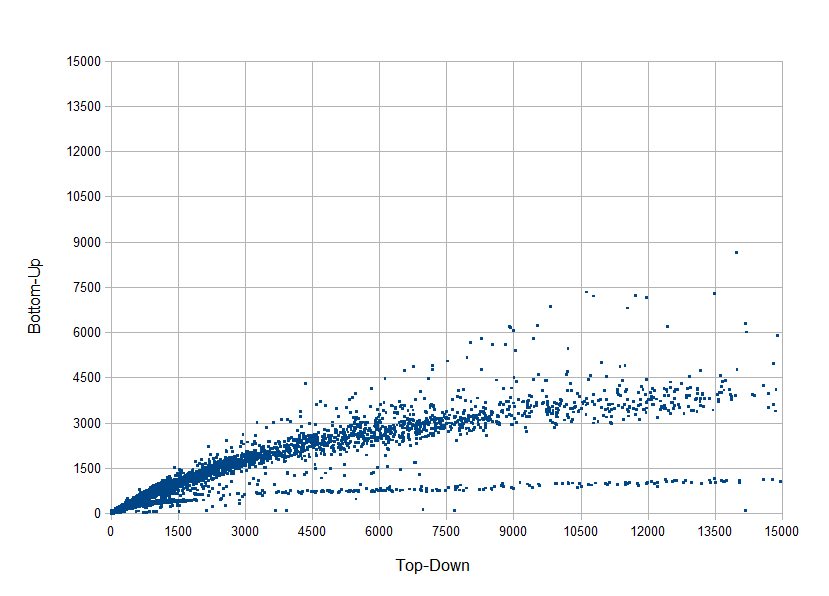
\includegraphics[scale=0.5]{Figures/TD_vs_BU-scatter.png}
	\caption{Average space measures of Bottom-Up and Top-Down heuristics}
	\label{fig:BUvsTD}
\end{figure}
  \BWP{What do you mean by ``average space measures'' of a heuristic? What exactly is each dot in this scatter plot?}

\section{Conclusions and Future Work}

Bruno


\vspace{-10pt}
\paragraph{Acknowledgments:}

\bibliographystyle{splncs}
\bibliography{biblio}


\end{document}

% vim: tw=100
